\documentclass{article}
\usepackage{amsthm}
\usepackage{amsmath}
\usepackage{graphicx}
\usepackage{multirow}

\newtheorem{problem}{Problem}

\begin{document}
\title{Sets, Maps, and Implementation}
\author{Henry Z. Lo}
\maketitle

\section{Set and Map ADTs}
Sets and maps are abstract data types (ADTs), which means that they are defined by their behaviour, not their implementation.  Since run-time depends on implementation, we will not analyse how fast operations are on sets and maps until later.

\subsection{Sets}
A \textit{set} is defined as a collection of distinct objects.  This corresponds to the mathematical definition of a finite set.

Since each element is distinct, this means that there cannot be duplicates.  \verb|{"dog","cat","rabbit"}| is a set, but \verb|{"dog","cat","rabbit","cat"}| is not.

Note that the definition says nothing about ordering.  This can lead to odd behavior, e.g. creating the same set twice may yield different element orders.

\subsection{Maps}
A \textit{map} is defined as a set of pairs.  The two elements of the pair are usually referred to as \textit{key} and \textit{value}.  Keys must be unique.

As a set, maps don't need to define ordering \textit{between} pairs; however, the ordering \textit{within} a pair is important, i.e. the pair \verb|(a,b)| is not equal to \verb|(b,a)|.

Example of a map: \verb|{("name","Charles"), ("job","Cook")}|.  This is not a map: \verb|{("name","Charles"), ("job","Cook"), ("name","Judith")}|

\section{Interfaces}
\subsection{Set interface}
Remember the Java Collection interface?  It defines basic operations required of collections, the important ones being:
\begin{itemize}
\item \verb|boolean add(E e)|, which puts \verb|e| into the collection. \verb|E| is the parameterized class, i.e. the type of object the collection contains.
\item \verb|boolean contains(E e)|.
\item \verb|boolean remove(E e)|.
\item \verb|int size()|, which counts the number of elements in the collection.
\item \verb|Iterator<E> iterator()|, which returns an iterator over the collection elements.
\end{itemize}

There are other methods in the interface, but these are the core.  The Collection interface already defines everything a set can do.  Thus, we can define a Set interface as such:
\begin{verbatim}
public interface Set<E> extends Collection<E> {
}
\end{verbatim}
However, we need to keep in mind that any class that implements \verb|Set| cannot allow duplicate entries.

\subsection{Map interface}
The map interface in Java shares some commonalities with collection, but are not otherwise related.  Table \ref{MapCollectionTable} compares the two interfaces side by side.

\begin{table}
\centering
\begin{tabular}{|l|ll|}
\hline
           & Map & Collection \\
\hline
Inserting & \verb|put(K key, V value)|     & \verb|add(E e)| \\
\hline
\multirow{2}{*}{Checking} 
          & \verb|containsKey(Object k)|   & \multirow{2}{*}{\texttt{contains(E e)}} \\
          & \verb|containsValue(Object v)| & \\
\hline
Retrieving
          & \verb|get(Object k)|   & not needed \\
\hline
Removing
          & \verb|remove(Object k)|   & \verb|remove(Object o)| \\
\hline
          & \verb|entrySet().iterator()| & \\
Iterating & \verb|keySet().iterator()|   & \verb|iterator()| \\
          & \verb|values().iterator()|   & \\
\hline
\end{tabular}
\caption{A comparison of some functions of the map and collection interfaces. \label{MapCollectionTable}}
\end{table}

Even though a map can be thought of as a type of set, in Java they are not related.   This is because maps are not merely sets of pairs; they are used in very specific ways, i.e. keys serve as an index, and values serve as the data being stored.  

This is evident in the retrieval and removal functions in maps.  There is no removal function like this in Collection.

Note also that there are two parameterized classes, \verb|K| and \verb|V| in map, whereas collection has one.

\section{Implementations}
Both sets and maps can be implemented using hash tables or trees.  Both hash tables and trees require an index.  In the case of a set, this is the object being stored.  In the case of a map, it is the key.  Otherwise, the way trees and hash tables are used to implement maps and sets are very similar.

\subsection{Time complexity}
Time complexity of basic operations for both hash and tree implementations is  given in Table \ref{complexity}.  As discussed in the previous lecture, most basic operations can be done in constant time in hash implementations.  You should have learned from CS210 that tree implementations generally take $O(\log n)$ time.

\begin{table}
\centering
\begin{tabular}{|l|cc|}
\hline
           & Hash implementation & Tree implementation \\
\hline
Insert & $O(1)$ & $O(\log n)$ \\
Retrieve & $O(1)$ & $O(\log n)$ \\
Remove & $O(1)$ & $O(\log n)$ \\
Iterate & $O(n)$ & $O(n)$ \\
Sort & $O(n \log n)$ & $O(n)$ \\
First/last & $O(n)$ & $O(\log n)$ \\
\hline
\end{tabular}
\caption{Complexity of basic operations on TreeSets/TreeMaps and HashSets/HashMaps. \label{complexity}}
\end{table}

\subsection{Ordering}

The main benefit of tree implementations is that they sort data.  This yields several benefits:
\begin{itemize}
\item Getting first and last elements is done simply by finding the leftmost and rightmost child, respectively (see Figure \ref{bst}).
\item Getting elements sorted can be done with a left-to-right depth first search.
\end{itemize}

\begin{figure}
\centering
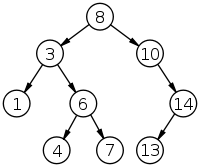
\includegraphics[scale=0.8]{bst.png}
\caption{A binary search tree, a common tree implementation. \label{bst}}
\end{figure}

For hash tables, there is no inherent ordering - thus, finding ordered elements requires iterating over all elements, and returning a sorted set requires running a sorting algorithm.

\subsection{Other considerations}

Trees need to be balanced periodically.  As hash tables grow, they must be rehashed.

Trees are more space efficient than hash tables, which must contain empty spots to reduce the probability of a collision.

Hashes contain some parameters, such as the initial capacity (how many slots) and load factor (what percentage of elements before rehashing).  These may need to be varied in order to optimize performance.  Trees don't have such parameters.

For the same data, hash tables may have different orderings; orderings may also change as hash tables get rehashed.  In other words, hash tables are less stable.  Trees are usually constructed deterministically.

\begin{problem}
You are programming software on a wristwatch.  You need to store lots of data, but do not have much memory.  Which data structure implementation would you use?
\end{problem}

Hash implementations are not memory efficient - they can take up to twice as much space as the number of elements you need to store.  Use a tree implementation.

\section{HashMap}
Let's actually implement HashMap using chaining to resolve collisions.

\subsection{Attributes}
There only needs to be the data structure, which can be an array (or ArrayList) of LinkedLists of Entries.  Each entry is a key / value pair of the generic types \verb|K| and \verb|V|.  Let's call the data structure \verb|entries|.

\begin{verbatim}
ArrayList<LinkedList<Entry<K,V>>> entries;
\end{verbatim}

The Entry class should be very bare, containing only the key and value attributes, a constructor, and getter methods.

Technically, if you don't care about storing keys, you can just have an ArrayList of LinkedList of generic types.  In this case you would not be able to implement \verb|keySet|, \verb|containsKey|, etc.  We continue assuming the first implementation.

\subsection{Constructor}
The constructor needs to take as a parameter a default size.  If we plan to rehash the table when it grows too large, then there also needs to be a load factor threshold.

\subsection{Methods}

Assume we have a \verb|hash| function, which returns a valid index.  For a map we need to implement the following methods:
\begin{itemize}
\item \verb|put(K key, V value)|: first get the appropriate list from the key, then add the new Entry object created from key and value.
\begin{itemize}
\item \verb|LinkedList<Entry<K,V>> myList = entries.get(hash(key));|
\item \verb|myList.add(new Entry(key, value));|
\end{itemize}
\item \verb|containsKey(Object k)|: calculate \verb|myList|; use \verb|contains| instead of \verb|add|.
\item \verb|containsValue(Object v)|: this requires iterating over the whole table, because we do not hash values.
\item \verb|get(Object k)|: calculate \verb|myList|, iterate.
\item \verb|remove(Object k)|: calculate \verb|myList|, then use \verb|remove|.  Note that this essentially iterates over the list.
\end{itemize}

\subsection{Iterator}
For \verb|entrySet(), keySet(), values()|, you need to return a single iterator.  However, if we just call iterator, we will just get an iterator for LinkedLists.  We need an iterator for items.

Given an iterator of collections called \verb|inputs|, and an inner iterator  \verb|inner|:
\begin{verbatim}
public boolean hasNext() {
  while (!inner.hasNext() && inputs.hasNext()) {
    inner = inputs.next().iterator();
  }
  return inner.HasNext();
}

public T next() {
  if (!hasNext())
     throw new NoSuchElementException();
  return inner.next();
}
\end{verbatim}
\end{document}